\documentclass[11pt]{report}
%\usepackage[german]{babel}

%(Rust) Code Snippets
\usepackage{minted}
\usemintedstyle{borland}

\setminted{
    framesep=2mm,
    fontsize=\footnotesize,
    linenos
}
%\usemintedstyle{trac}

%table cells
\usepackage{makecell}

%chapter style
\usepackage{titlesec}
\titleformat{\chapter}{\normalfont\huge\textbf}{\thechapter.}{20pt}{\huge\textbf}

%References as a Chapter
\usepackage[nottoc,numbib]{tocbibind}

%Graphs
\usepackage{pgfplots}
\usepackage{subcaption} % For subfigures
\pgfplotsset{width=15cm,height=7.5cm,compat=1.18}
\begin{comment}
    \usepgfplotslibrary{external}

    \usetikzlibrary{external}
    \tikzexternalize[
        failed ref warnings for={%
        \ref,%
        %\cite,% DISABLE THIS
        \pageref},
        shell escape=-shell-escape]
    \tikzset{external/system call={
        pdflatex -shell-escape -interaction=batchmode -jobname "\image" "\texsource"
    }}



    \tikzset{external/aux in dpth=false}




    \tikzset{
        png export/.style={
            % First we call ImageMagick; change settings to requirements
            external/system call/.add={}{& magick.exe -density 300 "\image.pdf" "\image.png"},
            % Now we force the PNG figure to be used instead of the PDF
            /pgf/images/external info,
            /pgf/images/include external/.code={
                \includegraphics[width=\pgfexternalwidth,height=\pgfexternalheight]{##1.png}
            },
        }
    }
\end{comment}


%CSV files
\usepackage{filecontents}

% For adjusting margins locally
\usepackage{changepage}

% Adjust spaces locally
\usepackage{setspace}

%Definitions
\usepackage{amsthm}
\usepackage{mdframed}

\NewDocumentCommand\newmdtheoremenvnonumber{O{} m m }{%
    \newtheorem*{#2}{#3}
    \BeforeBeginEnvironment{#2}{%
        \begin{mdframed}[#1]}%
    \AfterEndEnvironment{#2}{%
        \end{mdframed}}%
}

\newmdtheoremenvnonumber{mydefinner}{\mydeflabel}
\newcommand{\mydeflabel}{}
\newenvironment{mydef}[1]
{\renewcommand\mydeflabel{#1}\begin{mydefinner}}
{\end{mydefinner}}

\newcommand{\attribution}[1]{\textup{(#1)}}


%Citations
\usepackage[style=authoryear, backend=bibtex, urldate=long, sorting=none, defernumbers=true,autocite=superscript]{biblatex}
\addbibresource{refs.bib}
\usepackage{csquotes}


%Math Library
\usepackage{amsmath}

%Images Library
\usepackage{float}
\usepackage{graphicx}
\graphicspath{ {./images/} }

%General Layout
\usepackage{geometry}
\geometry{
    a4paper,
    left=20mm,
    right=20mm,
    top=30mm,
    bottom=30mm,
%    total={6in, 8in}
}
% To adjust figure placement
\usepackage{adjustbox}


%Background image
\usepackage[pages=some]{background}

%Liks of TOC
\usepackage{hyperref}
%\usepackage{lstmisc}
\usepackage{holtxdoc}
\usepackage{pgfregressiontest}
\usepackage{hhline}

\hypersetup{
    colorlinks,
    linkcolor={blue!50!black},
    citecolor={blue!50!black},
    urlcolor={blue!80!black}
}


\backgroundsetup{
    scale=1,
    color=black,
    opacity=1,
    angle=0,
    contents={%
    \hspace*{13.5cm}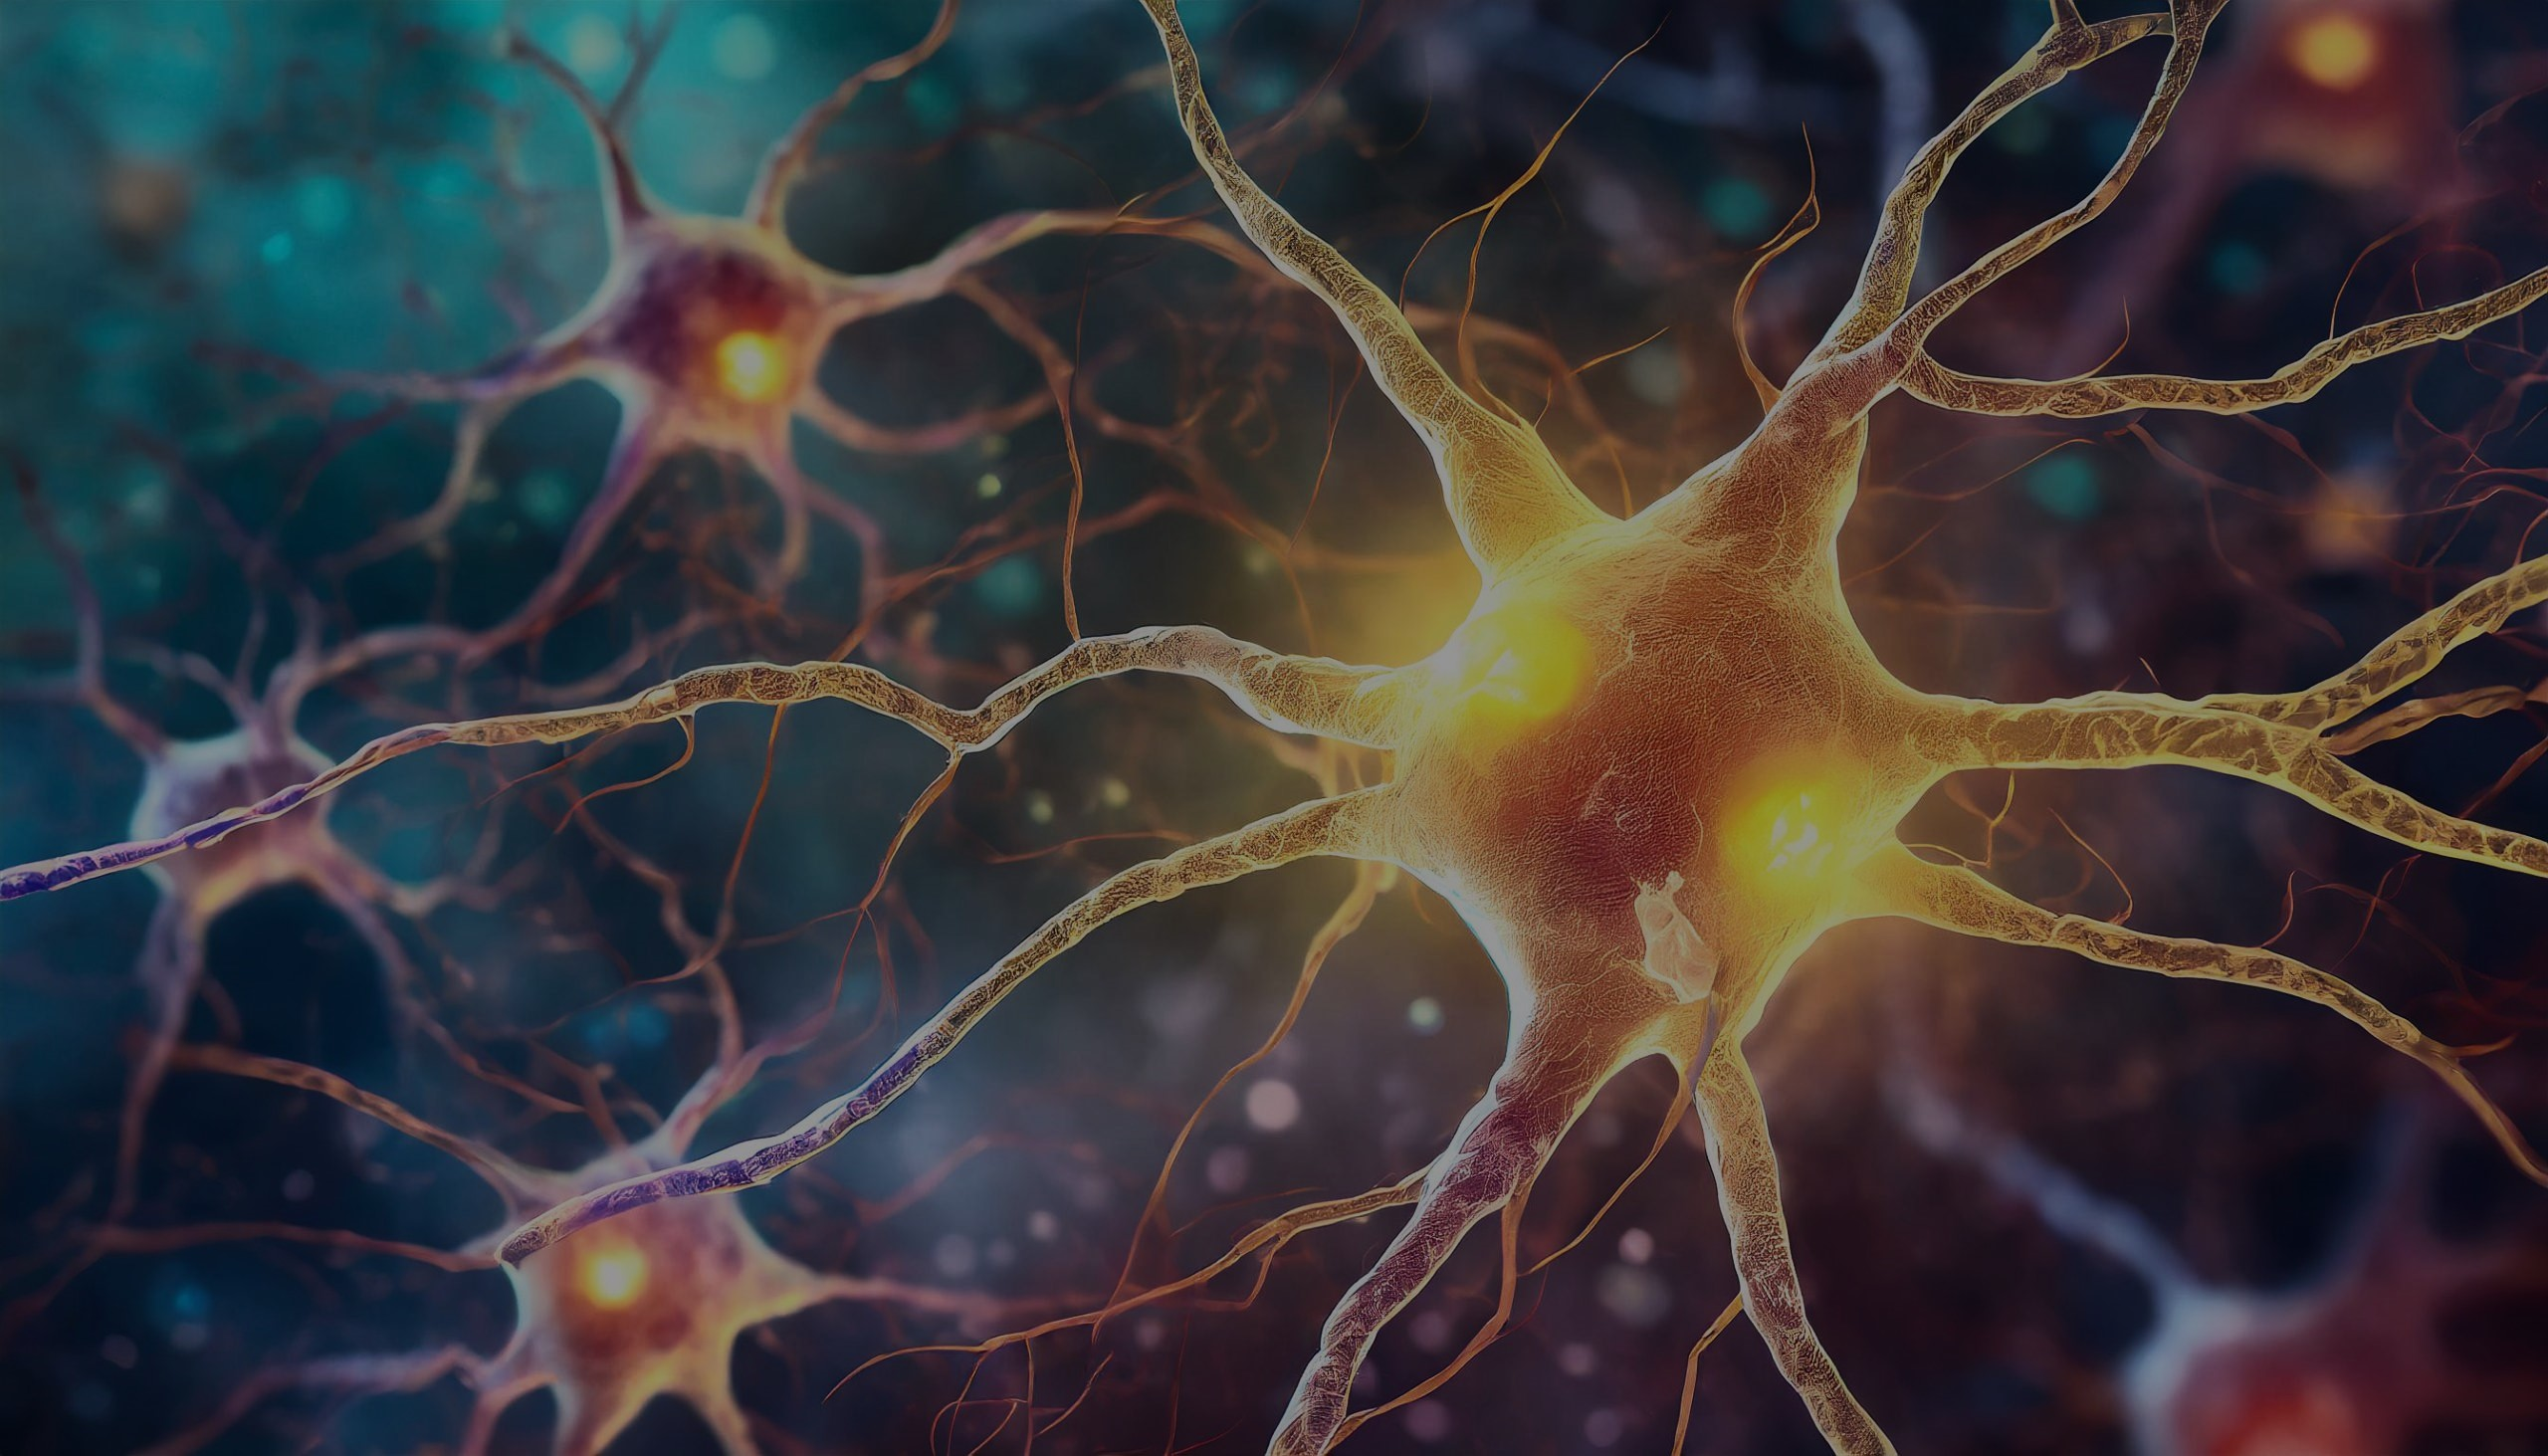
\includegraphics[width=3\paperwidth,height=\paperheight]{abstract_neurons3}
    }%
}


\begin{document}
    \pagenumbering{gobble}
    \begin{titlepage}
        \newgeometry{top=5mm, bottom=10mm, left=15mm, right=15mm}
        \BgThispage
        \color{white} {
            \begin{center}
                \Large \textsc{Matura Thesis}\\Kantonsschule Hohe Promenade\\
                \rule[0.1cm]{16.5cm}{0.1mm}\\
                \vspace{3cm}
                \Huge \textbf{ \textsc{Evolutionary Neural Networks: \\Designing a NEAT-Inspired Algorithm \\for Strategic Game Learning}}\\
                %\vspace{0.8cm}
                %\Large \textit {Implementation and Study of \\Evolutionary Neural Networks}\\
                \vspace{3cm}
                \rule[0.1cm]{16.5cm}{0.1mm}\\
            \end{center}
            \vspace{12cm}\\
            \begin{minipage}[t]{0.47\textwidth}
                \large\textbf {Thesis By:}\\
            \end{minipage}
            \hfill
            \begin{minipage}[t]{0.47\textwidth}
                \raggedleft
                \large\textbf {Lucien Kissling 6e}\\
            \end{minipage}
            \begin{minipage}[t]{0.47\textwidth}
                \large \textbf {Year:}\\
            \end{minipage}
            \hfill
            \begin{minipage}[t]{0.47\textwidth}
                \raggedleft
                \large \textbf {2025}\\
            \end{minipage}
            \begin{minipage}[t]{0.47\textwidth}
                \large \textbf {Supervisor:}\\
            \end{minipage}
            \hfill
            \begin{minipage}[t]{0.47\textwidth}
                \raggedleft
                \large \textbf {Timo Schenk}\\
            \end{minipage}
            \begin{minipage}[t]{0.47\textwidth}
                \large \textbf {Co Examiner:}\\
            \end{minipage}
            \hfill
            \begin{minipage}[t]{0.47\textwidth}
                \raggedleft
                \large \textbf {Dr. Arno Liegmann}\\
            \end{minipage}
            \vfill
        }
        \clearpage
        \restoregeometry
    \end{titlepage}
    \newpage
    \hspace{10cm}
    \newpage
    \vspace*{5em}
    \begin{doublespace}
        \begin{center}
            \textbf{Abstract.}
        \end{center}
        \\
        This thesis explores the design and implementation of Evolutionary Neural Networks (ENNs) inspired by the NEAT algorithm.
        ENNs optimize neural network weights, biases, and topologies using evolutionary computation.
        The game Nim and a simplified version with only one instead of multiple stacks are used as a benchmark of the ENN algorithm to test the effect of different parameters and features on performance.
        The research shows that ENNs can successfully learn to play simple games like Single-Stack Nim but struggle with more complex games like multi-stack Nim.
        Challenges include overcoming local minima, tuning the ENN parameters correctly, and dealing with limited computations.
        \\
        \textbf{Results.}
        The results show that ENNs achieve 100\% accuracy for simple Nim, a single-stacked version of the game, with stack sizes up to 1000 matches, revealing the importance of using correct output encoding.
        In the multi-stacked Nim game, ENNs reach an accuracy of 90\% for the configuration with 2 stacks with 4 matches each, however, they could not find the perfect moves for all game states because of local minima.
        \\
        \textbf{Keywords.}
        Evolutionary Neural Networks, NEAT Algorithm, Machine Learning, Game Learning, Nim Game, Evolutionary Computation.

        \newpage
        \vspace*{5em}
        \begin{adjustwidth}{2cm}{2cm}
            \textit{
                I want to express my fullest gratitude to my parents for their support on my journey and especially during my thesis, where their help was crucial for the completion of this project.
                \\ \\
                I would also like to extend my sincerest thanks to my supervisor Timo Schenk for sharing his large expertise in the field of machine learning and his invaluable feedback, which were essential for this work.
                \\ \\
                Lastly, I want to express my deepest gratitude to Jan Wilhelm for introducing me to the fascinating world of computer science, which I have grown to love, and for assisting me with many technical challenges.
            }
        \end{adjustwidth}
    \end{doublespace}
    \newpage

    \pagenumbering{arabic}
    \setcounter{page}{5}
    \tableofcontents


    \chapter{Introduction}\label{ch:introduction}


    \section{Preface}\label{sec:preface}
    Ever since I got into computer science a few years ago, I was fascinated by the idea of algorithms that solved various problems.
    Therefore, I participated in the SOI (Swiss Olympiad in Informatics) where we were taught everything about developing and programming algorithms and their data structures.
    \\ \\
    In recent years although, a new field of computer science has gained a lot of attention, where these algorithms are not programmed by humans, but evolved by a computer.
    This field called machine learning immediately got my excitement and two years ago a friend of mine and I had our first practical experience with it.
    I developed a simple neural network, which helped us predict the color of a lego brick in front of a color sensor based on the RGB values in various lighting conditions.
    \\ \\
    A neural network (NN) forms the basis of most machine learning models and I will therefore explain it in much detail in the following chapters.
    In simple terms however, a NN is a strongly simplified artificial model of the human brain consisting of an interconnected web of neurons through which information flows and gets computed.
    \\ \\
    Although the NN I developed two years ago already learned on its own, I still had to provide and label data for it to learn from.
    This meant that I had to manually scan the RGB values of the lego bricks and assign them the color they represented.
    In this case, this was the most efficient solution, however there are cases where you train a model where such data is unavailable or you simply want them to develop their own approach for a problem without predefined solutions.
    That is how I got to my matura thesis, which aims to develop such ML models that learn without labeled data and use these models to learn games.


    \section{Thesis Statement}\label{sec:thesis-statement}
    This thesis explores the field of neural networks (NNs) capable of learning without human-provided data, known as unsupervised learning.
    The focus is on evolutionary neural networks (ENNs), which combine neural networks with evolutionary computation.
    \\ \\
    In this thesis, a simplified implementation of ENNs is developed and trained on board games.
    The research investigates the effects of varying parameters and features on the learning process and evaluates the algorithm’s performance in comparison to other machine learning approaches.
    This project draws inspiration from the NEAT Algorithm, introduced by Kenneth O. Stanley and Risto Miikkulainen in 2002, which uses a minimal initial structure that evolves complexity over time.\footcite[p.105-106]{Neat_02}
    As a benchmark, the ENNs are trained to play the game Nim, where players alternately remove matches from stacks, and the winner is the one who avoids taking the last match.
    \\ \\
    In specific, this Thesis addresses following questions:
    \begin{itemize}
        \item How can evolutionary neural networks (ENNs) be developed that learn to play simple games?
        \item How do different parameters and features of ENNs affect the learning process?
    \end{itemize}


    \chapter{Background}\label{ch:background}


    \section{Neural Networks (NNs)}\label{sec:neural-networks-(nns)}

    As previously mentioned in the Preface, an artificial neural network (ANN or NN) is a mathematical model for data processing, initially inspired by the structure of the brain.
    Therefore, a brief overview of how a brain functions is presented next.

    \subsection{Neurons in the Brain}\label{subsec:neurons-in-the-brain}
    Inside the brain, around 86 million neurons\footcite{caruso_23} form connections to each other through which they activate other neurons with electric and chemical signals.
    In a neuron, the signals of connected neurons add up and when they reach a certain threshold, the neuron is activated and fires a new signal to its own connections\footcite{Newman_23}.
    The neuron then resets after a certain amount of cooldown time.
    \\
    With this web of neurons inside the brain, animals can process the information from nerve signals from the body and output them again as nerve signals instructing the body.

    \subsection{Feed Forward Neural Networks (FNNs)}\label{subsec:feed-forward-neural-networks-(fnns)}
    So how can these ideas about neural networks learned from the biology of a brain be applied to a program that runs on a computer?
    The first step is to simplify the chaos of neurons in the brain and organize them into layers of neurons.
    These layers consist of an input layer, an output layer and optional so-called hidden layers in between.
    As a next step, the neurons in each layer are connected to those in subsequent layers, typically limited to connections with the nearest layer.\footcite{Hardesty2017}
    \\
    Now, the structure of a neural network looks something like this:
    \begin{figure}[H]
        \centering
        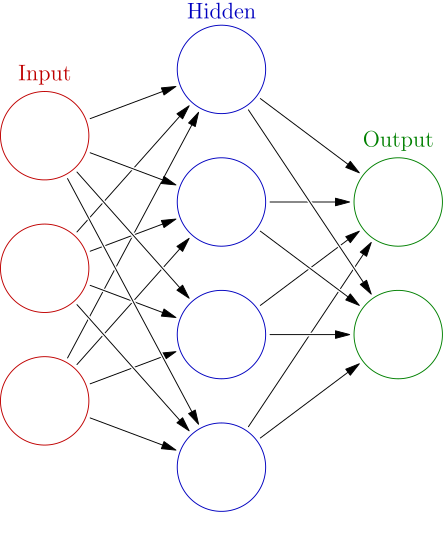
\includegraphics[width=0.25\textwidth]{nn_simple_1}~\caption{A simple Feed Forward Neural Network (FNN) with three layers: Input, Hidden and Output.\footnote{\cite{nn_simple_img_1}}}
        \label{fig:nn_simple_1}
    \end{figure}

    To describe the specific structure of a NN, the term topology is used\@.
    \begin{mydef}{Neural Network Topology}
        The topology of a neural network is its distinct arrangement of neurons, layers and the connections between the neurons.\footcite{Miikkulainen2010}
        \label{definition:Topology}
    \end{mydef}
    For the neural network to perform functions, a weight needs to be assigned.
    This weight value ranges from -1 to 1 and can be thought of as the strength of a connection between neurons.
    \\
    In terms of computer science, this structure now resembles a directed, weighted graph, which is why the neurons are called nodes and their connections edges.
    \begin{mydef}{Nodes/Edges}
        In a neural network, a node receives, computes and sends information, whereas an edge forms the connections between nodes to exchange information.\footcite{Sanchez-Lengeling2021}
        \label{definition:Nodes-Edges}
    \end{mydef}
    \\ \\
    The computation process of information by a neural network can be illustrated through the example of a computer vision NN that recognizes digits in a black-and-white image.
    As a first step, the input is encoded into values that correspond to the nodes of the input layer.
    In the example of a computer vision NN, the brightness values of the single pixels might directly represent the nodes of the input layer.
    \\
    Then, the algorithm iterates through all input nodes to identify its connected edges.
    For each of these edges it multiplies its weight by the value of the input node and adds the result to the node on the receiving end.
    \\
    After iterating through all the nodes of one layer, it moves to the next layer.
    At this point, the value of the nodes in the current layer is the sum accumulated by the values of all connected nodes multiplied by the weight of that connection:
    \begin{equation}
        v_x = \sum_{i=0}^{N}v_i * w_i\label{eq:sum_connected_nodes}
    \end{equation}
    Where:
    \textit{
        \begin{itemize}
            \item $v_x$ is the value of the current node
            \item N is the number of connected nodes
            \item $v_i$ is the value of the connected node i
            \item $w_i$ is the weight of the edge connecting the current node to node i
        \end{itemize}
    }

    Additionally, some algorithms add a bias value $r_x$ ranging from -1 to 1 onto the value of the nodes.\footcite{IBMNeuralNetworks}
    Finally, an activation function\footcite{Baheti2021} $\sigma(x)$ is applied to the value of the nodes to fit the value of the node inside a preferred range.
    This activation function can also be thought of as the threshold of stimulation for a neuron to fire.
    Two examples for activation functions are:
    \begin{itemize}
        \item Sigmoid Function: $\sigma(x) = \frac{1}{1 + e^{-x}}$
        \item Rectified Linear Unit (ReLU): $\sigma(x) = \max{0, x}$
    \end{itemize}
    Plot of the activation functions:
    \\ \\
    \begin{center}
        \begin{tikzpicture}
            \begin{axis}
                [
                xmin=-6,
                xmax=6,
                ymin=0,
                ymax=6,
                ytick distance = 1,
                xtick distance = 1,
                minor tick num=1,
                axis lines = left,
                line width = 1.5pt,
                grid=both,
                major grid style={line width=0.8pt,draw=gray!50},
                minor grid style={line width=0.4pt,draw=gray!20},
                xlabel = \(x\),
                ylabel = {\(\sigma(x)\)}
                ]
                % First plot (Sigmoid)
                \addplot[
                    domain=-10:10,
                    color=red,
                    samples=1000,
                ]{1/(1 + e^-x)};

                % Second plot (ReLU)
                \addplot[
                    domain=-10:10,
                    color=blue,
                    samples=1000,
                ]{max(0,x)};

                % Define the legend after all plots have been added


                \legend{Sigmoid, ReLU}

            \end{axis}
        \end{tikzpicture}
    \end{center}

    \\ \\
    The complete function for the value of one node is therefore:
    \begin{equation}
        v_x = \sigma\left(\sum_{i=0}^{N}v_i * w_i + r_x\right)\label{eq:value_node}
    \end{equation}
    Where (additionally to equation~\ref{eq:sum_connected_nodes}):
    \textit{
        \begin{itemize}
            \item $r_x$ is the bias of the node
            \item $\sigma$ is the activation function
        \end{itemize}
    }

    Now this value $v_x$ is again sent through its connections to nodes in the upcoming layers.
    After iterating through all the nodes and layers of the neural network (NN), the process reaches the final layer of the NN, where the computed output can be read out.
    This output is encoded in node values, as was done with the input, and therefore requires decoding to obtain the final result.
    In the example of a digit-detecting NN, 10 output nodes could be used, each representing one digit.
    The result could then be decoded by identifying the output node with the highest value as the result.
    This kind of output encoding, where all possible results are assigned their own node, is referred to as one-hot output encoding\footcite{Brownlee2020}.
    With one-hot output encoding, the values of the output nodes can be interpreted as a the neural networks certainty for a specific result to be correct.

    \subsection{Remark: Functioning of NNs}\label{subsec:remark-about-the-funtioning-of-nns}
    Having established how a neural network operates, it is important to understand why this type of algorithm is considered revolutionary in the field of computer science.
    \\ \\
    An algorithm processes an input with a set of functions applied in a certain order to calculate an output.
    Traditionally, a computer algorithm gets programmed with the help of mathematical operations, logic functions, loops, system functions, and data structures, which are then converted into binary code for the processor.
    Of course, this also applies in the context of NNs.
    However, there is also a third layer of abstraction on top, which simulates the functioning of a brain with neurons.
    Since the traditional algorithm only enables the neurons of a NN, the third neuron-based layer is what computes the actual function of the NN. Therefore, NNs resemble more the functioning of a brain than a traditional algorithm.
    \\ \\
    This difference has implications for the functioning of an NN: Traditional algorithms represent actual mathematical calculations and are therefore deterministic.
    With NNs, the algorithm is based on different parameters for nodes and edges, which make it an unpredictable black box.
    In the top layer of abstraction, there are no concrete functions but only neuron activation that approximates a function instead.
    This means it is hard to prove a neural network to always be accurate and is also the reason why the result of NNs is often called its prediction. \footcite{springer_blackbox}%nature_blackbox,

    \begin{mydef}{NN Prediction}
        The output of a neural network is referred to as its prediction for a given input.\footcite{Warudkar2020}
    \end{mydef}

    \subsection{An Example of NN learning: Backpropagation}\label{subsec:an-example-of-nn-learning:-backpropagation}
    It has already been established how a neural network with specific parameters generates a prediction for a given input.
    This however raises the question: how can parameters encoding the structure, weights, and biases of the neural network be determined?
    The solution lies in using machine learning, which trains the model to perform a specific task using training data.
    \begin{mydef}{Machine Learning}
        Machine learning (ML) is a branch of artificial intelligence that focuses on optimizing artificially intelligent models to solve a given problem.\footcite{IBM_Machine_Learning}
    \end{mydef}
    One machine learning algorithm for NNs is called backpropagation, which is one of the simplest and most efficient methods to train a NN.\footcite{Al-Masri2024}
    Backpropagation works using a training and test set containing labeled data for a problem.
    \begin{mydef}{(Un)labeled Data}
        Labeled data for a machine learning problem is a set of data with sample problems and the respective solutions.
        Unlabeled data instead only contains the sample problems.\footcite{IBM_Data_Labeling}
    \end{mydef}
    The machine learning process of backpropagation begins with a neural network that has a fixed topology and random weights and biases.
    First, the NN is given the training problems for which it will generate random predictions.
    These random predictions are then refined using the sample solutions.
    This is done by looping back through the NN from the output layer to the input layer, always adjusting the weights and biases in a way that the NN would finally make the right prediction for this problem.
    However, the NN shouldn't be adapted only to a single problem but make accurate predictions for the whole training set and unknown problems.
    To therefore prevent overcorrecting a NN for single problems, a learning rate significantly smaller than 1 is applied to the corrections.
    \\ \\
    The NN is trained on the whole training set for many generations, until the NN starts to make accurate predictions for all problems.
    To evaluate the performance on unknown problems, a separate test set, which the NN hasn't been trained on, can be used.


    \section{Evolutionary Computation (EC)}\label{sec:evolutionary-computation-(ec)-&-genetic-algorithms-(gas)}
    The focus now shifts to the machine learning technique this thesis focuses on.
    Once again, nature serves as inspiration:
    \begin{mydef}{Evolutionary Computation}
        Evolutionary Computation (EC) is an Algorithm that optimizes a set of parameters for a problem with the help of natural selection.\footcite{virtusa2024}
    \end{mydef}
    Evolutionary computation (EC) is often employed in situations where the optimal parameters for a function cannot be directly calculated, but the performance of a given parameter set can be evaluated.
    One example scenario involves a large dataset of points representing an unknown polynomial function with added noise and outliers.
    To determine the parameters of the underlying polynomial, EC can be utilized to identify the best-fitting parameters.
    The following shows how EC achieves this optimization.
    \\ \\
    The process starts with an initial population of agents with random parameter sets.
    EC then repeats following steps, forming a new generation of the population in each iteration\footcite{Sathyabama20}:
    \begin{itemize}
        \item \textbf{Fitness evaluation:} First, EC assesses the performance of each agent, defined by its parameters, in the given problem.
        This performance is referred to as the agent's fitness, which can be evaluated either objectively through a cost function or relatively with a competition between agents.
        In the given example, the cost function might check the prediction of the NN for the given data points, calculate the absolute differences between the prediction and the values of the data points, and use the total sum of these differences as the cost.
        \item \textbf{Selection:} As a next step, the agents that performed well are selected to be part of the next generation.
        \item \textbf{Reproduction:} The selected agents are then replicated by directly copying their parameters (non-mating) or by merging parameters from different agents (crossover).
        \item \textbf{Mutation:} In each new generation, the parameters of the agents are mutated, either by completely replacing certain parameters with new random parameters or by shifting the existing parameters by a random value.
    \end{itemize}
    After a certain number of generations, the EC algorithm will have found best performing set of parameters for a given problem.

    \subsection{Gradient Descent}\label{subsec:gradient-descent}
    As established in the previous section, EC begins with an initial population of agents with a random set of parameters.
    The fitness of these agents is determined using a cost function.
    Agents with relatively low cost (or high fitness) survive the round and are replicated, mutated and again selected by cost.
    \\ \\
    This whole process strongly resembles a ball rolling down a hill in some terrain.
    At any given point on the terrain, the ball moves in the direction of the steepest descent (ignoring the inertia of the ball).
    Applying this analogy to EC, the parameters for a function can be imagined as the horizontal coordinates for the ball meanwhile the cost of these parameters correspond to the height at that location.
    Mutations produce parameter sets that are close to the original, resembling neighboring points on the terrain.
    As the ball rolls down to the lowest neighboring point in any step, EC again chooses the set of parameters with the lowest cost every cycle.
    This is why the machine learning process is referred to as gradient descent, as the algorithm evaluates all neighboring points and then follows the direction with the lowest cost and therefore steepest gradient\footcite{ibm2024}.

    \subsection{Initial Position \& Local Minima}\label{subsec:initial-position-&-local-minima}
    The ball analogy provides insights into the functioning of the EC learning process, which can be understood by visualizing a hill with each a shallow and a deep valley next to it.
    Depending on which side of the hill the ball is placed in the beginning, it will roll in a different direction and end up in either of the two valleys, which have different heights.
    Therefore, following things can be derived:
    \begin{itemize}
        \item (Minor) differences in the starting position can result in large differences in the end position and the respective cost.
        \item Once a point with no downwards gradient is reached, innovation halts for that agent, even if there is a point with lower cost somewhere else.
        Such points are called local minima.
    \end{itemize}
    \begin{mydef}{Local Minimum}
        A local minimum is a point with minimal cost compared to its neighboring area and is therefore a halting point for gradient descent.\footcite{ayoosh2024}
    \end{mydef}
    The impact of starting position and local minima often pose a large problem for EC applications.
    Strategies to reduce the impact of such are therefore crucial for the algorithms success.


    \section{Evolutionary Neural Networks (ENNs)}\label{sec:evolutionary-neural-networks-(enns)}
    After having covered all the basics about neural networks and evolutionary computation, the two concepts are finally combined to create the algorithm this thesis focuses on.
    \begin{mydef}{Evolutionary Neural Networks}
        Evolutionary neural networks (ENNs) are neural networks that use an evolutionary algorithm called neuroevolution to optimize for its parameters for the NNs weights/biases and its topology.\footcite{enn22, neuroevolution19}
    \end{mydef}
    ENNs are useful for complex machine learning problems and also work for unlabeled training data as long as there is a fitness function.
    In the context of neural networks, evolutionary computation can be applied as follows:
    \\
    The parameters encoded by ENNs represent the weights, biases, nodes, and edges of a neural network.
    ENNs still follow the same core process of evolutionary computation:
    They start with a random population of NNs that are evaluated and selected based on a fitness function.
    The selected NNs are replicated (with crossover or non-mating) and finally mutated in following ways:
    \begin{enumerate}
        \item \textbf{Change weights/biases:} A new random value is set for the weight or bias of a random existing edge or node.
        \item \textbf{Shift weights/biases:} The value for an existing weight or bias of a random existing edge or node is altered by a random change but is kept close to the old value.
        \item \textbf{Add edges:} A new edge is added between two random, previously unconnected nodes.
        \item \textbf{Add nodes:} A new node is added in between of a random existing edge.
        The old edge is removed and two new edges with random weights are added between the new node and the two other nodes each.
        \item \textbf{Remove nodes/edges:} A random node or edge is removed in a way that doesn't cut off the input from the output layer.
    \end{{enumerate}}


    \section{The NEAT-Approach}\label{sec:the-neat-approach}
    As already stated in the thesis statement(\ref{sec:thesis-statement}), neuroevolution of augmenting topologies is an ENN machine learning algorithm developed by Kenneth O. Stanley and Risto Miikkulainen in 2002\footcite[p.105-106]{Neat_02}.
    NEAT evolves the topology, weights and biases of NNs at the same time, which makes it particularly suitable for tasks where the optimal network architecture is not yet known.
    One of its key innovations is that the initial population begins with NNs of lowest complexity and the NNs only increase topological complexity as it is useful for the problem.
    In specific, the NEAT algorithm starts with NNs that only have the nodes of the input layer connected to the nodes of the output layer.
    This design aims to produce more efficient neural networks by only increasing complexity when it leads to improved performance.
    The NEAT algorithm therefore only needs the mutations 1. to 4. shown in the last section(\ref{sec:evolutionary-neural-networks-(enns)}) and doesn't need to remove complexity (mutation 5.) as it is already minimal.


    \section{Games}\label{sec:games}
    The following section offers a brief overview of the games on which the ENNs will be trained.

    \subsection{Simple Nim}\label{subsec:simple-nim}
    This game is a simplified version of Nim, where two players take turns removing an arbitrary amount of matches from a single stack with some number of matches.
    The player who removes the last match loses.
    Therefore, the winning strategy simply is to remove all matches from the stack but one, forcing the opponent to remove the last match and therefore making them lose.

    \subsection{Nim}\label{subsec:nim}
    This game works similarly to Simple Nim with the difference that there are multiple stacks with matches.
    Now, the player who removes the last match from the last unemptied stack loses.
    The winning strategy for Nim involves a binary representation of the game state\footcite{rosenbloom2003} and is therefore mathematically much more complex, which forces the ENNs to learn more sophisticated strategies.


    \section{Related Work}\label{sec:related-work}
    The field of AI research in ENNs is largely studied and is often linked to games.
    The following table provides some examples of ENN models that have been tested on games:

    \footnotesize
    \begin{center}
        \hspace*{-2cm}\begin{tabular}{|| l l l l l ||}
                          \hline
                          \makecell{\textbf{Author(s) \& Year}} &
                          \makecell{\textbf{Model}} &
                          \makecell{\textbf{Game/Benchmark}} &
                          \makecell{\textbf{Computation}} &
                          \makecell{\textbf{Accuracy}} \\
                          \hline\hline
                          \makecell{\cite{Neat_02}} &
                          \makecell{NEAT} &
                          \makecell{Double Pole Balancing \\With Velocities} &
                          \makecell{3600 \\evaluations} &
                          \makecell{100\%} \\
                          \hline
                          \makecell{\cite{dama_22}} &
                          \makecell{NEAT} &
                          \makecell{Dama} &
                          \makecell{$>$5000 \\generations} &
                          \makecell{81.25\%\\(wins against humans)} \\
                          \hline
                          \makecell{\cite{go_98}} &
                          \makecell{SANE} &
                          \makecell{Go} &
                          \makecell{260 \\generations} &
                          \makecell{$>$75\%\\(vs Wally, 9$\times$9 board)} \\
                          \hline
                          \makecell{\cite{capture_02}} &
                          \makecell{Custom \\ENN} &
                          \makecell{Capture Game\\(subgame of Go)} &
                          \makecell{$>$100 \\generations\\(distributed)} &
                          \makecell{No significant \\progress yet} \\
                          \hline
                          \makecell{\cite{backgammon_07}} &
                          \makecell{Genetic \\ENN} &
                          \makecell{Backgammon} &
                          \makecell{256 pop,\\100–200 \\generations} &
                          \makecell{62.4\%\\(vs Pubeval)} \\
                          \hline
        \end{tabular}\hspace*{-2cm}
    \end{center}
    \normalsize
    Note:
    Although the amount of fitness evaluations is a more accurate representation of computation load than the amount of generations, in many cases the amount of fitness evaluations isn't indicated and cannot be derived.


    \chapter{Building an ENN}\label{ch:designing-an-enn}


    \section{Algorithm Design}\label{sec:algorithm-design}
    This section details how to use the concepts described in the last chapter(\ref{ch:background}) to build an evolutionary neural network that plays Nim.

    \subsection{Overview}\label{subsec:overview}
    As already mentioned in the thesis statement(\ref{sec:thesis-statement}), this project is written in the Rust programming language\footcite{rust23}.
    The source code and all test data can be found on this thesis' GitHub page\footcite{RustENN}.
    This project utilizes following Rust libraries:
    `rand` (version 0.9.0-alpha.2)\footcite{rand2024},
    `indicatif` (version 0.17.8)\footcite{indicatif2023},
    `csv` (version 1.3.0)\footcite{csv2023},
    `bincode` (version 1.3.3)\footcite{bincode2021},
    `serde` (version 1.0.209)\footcite{serde2024},
    and `rayon` (version 1.10.0)\footcite{rayon2023}.
    The code has been partially written by the AI coding assistant GitHub Copilot\footcite{github_copilot2021}.
    Every instance of artificially generated code has been thoroughly reviewed.
    \\ \\
    The codebase is divided into different modules as well as a bin folder containing main files.
    One module manages the ENN algorithm, while another handles the games that the ENNs are trained to play.
    The ENN module itself is further divided into two files:
    \begin{itemize}
        \item \textbf{agent.rs:} This file handles the NNs and the mutations on the NNs
        \item \textbf{population.rs:} This file handles the natural selection process and data saving
    \end{itemize}
    The game modules provide the problems for the NNs, handle the predictions of the NNs, and find the new game state after a move.
    It further includes an objective performance evaluation function to measure how well the NNs perform.
    \\ \\
    The following sections provide a bottom-up explanation of all functions, beginning with the neural network.
    The implementation uses Rust's structs, which are similar to classes in other programming languages.

    \subsection{Neural Network}\label{subsec:neural-network}
    The struct \textit{NeurualNetwork} (defined in agents.rs) most importantly contains a two-dimensional vector of nodes, which encodes all the information of the NN\@:
    \begin{minted}{rust}
    pub struct NeuralNetwork {
        [...] // redundant side data about the NN
        pub nodes: Vec<Vec<Node>>,
    }
    \end{minted}
    The vector inside (\mintinline{rust}{Vec<Node>}) represents a layer of the NN and the outside vector (\mintinline{rust}{Vec<Vec<Node>>}) contains all layers of the NN\@.
    A \textit{Node} contains its bias and a vector for the incoming and outgoing edges:
    \begin{minted}{rust}
    pub struct Node {
        pub bias: f64,
        //edges stored in an adjacency list
        pub incoming_edges: Vec<Edge>,
        pub outgoing_edges: Vec<Edge>,
    }
    \end{minted}
    An \textit{Edge} contains the weight of the edge and its input/output node:
    \begin{minted}{rust}
    pub struct Edge {
        input: [usize; 2],
        out: [usize; 2],
        weight: f64,
    }
    \end{minted}
    The most important functions of the \textit{NeuralNetwork} struct are:
    \begin{itemize}
        \item \mintinline{rust}{new(input_nodes: usize, output_nodes: usize) -> Self {}}, which initializes the NN with all input and output nodes connected to each other with random weights and biases.
        \item \mintinline{rust}{predict(&self, input: Vec<f64>) -> Vec<f64>}, which computes the output of the NN for a given input with the forward propagation algorithm described in~\ref{subsec:feed-forward-neural-networks-(fnns)}.
        \item \mintinline{rust}{activation_function(x: f64) -> f64}, which computes the neuron activation described in~\ref{subsec:feed-forward-neural-networks-(fnns)}.
        This implementation uses a variant of the \textit{ReLU} function.
        The linearity for inputs greater than zero in the \textit{ReLU} function allows for more variety of neuron activations, enhancing the flexibility and efficiency of the neural network.
        The chosen variant is the \textit{ELU} function, which addresses the issue of dead neurons encountered in \textit{ReLU} by permitting negative output values.
    \end{itemize}

    \subsection{Mutation}\label{subsec:mutation}
    The mutation of the NNs is handled in the \textit{Agent} struct (defined in agent.rs), which includes a NN, its fitness, and its rank:
    \begin{minted}{rust}
    pub struct Agent {
        pub nn: NeuralNetwork,
        pub fitness: f64,
        pub rank: isize,
    }
    \end{minted}
    The function \mintinline{rust}{mutate(&mut self, mutations: usize) -> Self {} } has a number of mutations as a parameter which it applies to the NN of the agent.
    For each mutation, it randomly selects one of the following mutations: Change weights/biases, Shift weights/biases, Add edges, Add nodes.
    All of these mutations have already been described in the last chapter(\ref{sec:evolutionary-neural-networks-(enns)}), although there are some implementation details to mention:
    \begin{itemize}
        \item When inserting a new node in between of two connected nodes (mutation 4.), the inserted node will be added to a random layer in between of the previously connected nodes.
        If the previously connected nodes are in neighboring layers, a new layer is created in between for the new node.
        \item The shift mutation adds to the initial value a random float in the ra nge 0.0 to 1.0 squared with a random sign.
        This gives us following function: \\
        $v_{new} = shift(v_{old}) = v_{old} + rand(-1, 1) * rand_{float}(0..1)^2$
        \item The amount of mutations performed per NN is randomly selected in a range defined by adjustable parameters (see section~\ref{subsec:enn-parameters}).
        \item The type of mutation that is performed is randomly determined for each mutation.
        A weight can be assigned to each mutation as a parameter, which represent its probability to be selected relative to the weights of other mutations (see again section~\ref{subsec:enn-parameters}).
    \end{itemize}

    \subsection{Evolutionary Computation \& inspiration by NEAT}\label{subsec:evolutionary-computation-&-inspiration-by-neat}
    The EC process starts with an initial population of new agents with NNs created by the \mintinline{rust}{NeuralNetwork::new()} function (described in~\ref{subsec:neural-network}).
    As per the NEAT algorithm's approach, the new NNs have minimal structure, where all input nodes are directly connected to all output nodes with no hidden layers.
    Random values area assigned for the weights and biases of the initial NNs.
    Subsequently, the steps of performance evaluation, selection and mutation are repeated every generation.

    \subsubsection{Competition}
    In the approach examined by this thesis, the fitness of agents is assessed by having them compete against one another in the games.
    However, allowing every agent to play every other agent is computationally too expensive since the needed time increases quadratically with the population size.
    To address this, a circular pairing algorithm is employed.
    This algorithm sets a predefined number of opponents for each agent to play against (see~\ref{subsec:enn-parameters}).
    For each of these predefined games, the algorithm generates a new pairing distance, which it then uses to pair each $\textrm{agent}_i$ with the $\textrm{agent}_{i+distance}$.
    It also checks that the distance isn't a multiple of any distance it had previously avoiding duplicate pairings between agents.
    Each game is played twice with both agents taking turns as the starting player while keeping the same initial state.

    \subsubsection{Fitness Evaluation}
    Now, the fitness function evaluates its fitness for each agents.
    The main idea for the fitness function is to simply count the number of wins an agent has scored during the competition.
    Of course, there are other possibilities to evaluate the performance of an agent that represent their performance more accurately.
    Still, the number of wins is used as fitness as this function is generally applicable to any game.
    Counting the number of wins doesn't require a deeper understanding of the game, which is very useful in games that are indeterministic.
    This also enables the ENNs to find their own new strategy for the game, which is finally the goal of machine learning.

    \subsubsection{Natural Selection}
    After the fitness evaluation, the performance of the current generation is evaluated (details in section~\ref{subsec:performance-tests}) before the new population is generated.
    The new population is made up by some portion of each of the following:
    \begin{itemize}
        \item \textbf{Agents from the last generation:}
        The main part of the new population will be drawn from agents from the old generation with high fitness.
        This works by selecting all needed agents randomly using the fitness of my agents as their relative probability of being drawn.
        The fitness can also be raised to some power to adjust the likelihood of survival for non-top-performing agents.
        \item \textbf{Random agents from the last generation:}
        Some fraction of the new population is made up of randomly selected agents from the last generation which might help counter a population with the top performing agents stuck in local minimum.
        \item \textbf{New random agents:}
        Another fraction of the new population is made up of newly generated, random agents which might help counter overly complex NNs and also local minima in a population.
        \item \textbf{Old best agents:}
        The last part of the new population is made up of best agents from previous generations which help counter populations stuck in a local minimum.
    \end{itemize}
    Now that the new population has been generated, the whole process can start over again.

    \subsection{ENN Parameters}\label{subsec:enn-parameters}
    As already mentioned in the thesis statement(\ref{sec:thesis-statement}), this research involves testing its implementation with several configurations of different parameters and then evaluate their performance with the stats described in the following section(\ref{subsec:performance-tests}).
    Here is a list of all possible parameters influencing the ENN algorithm:
    \begin{itemize}
        \item \textbf{General:} Size of the population
        \item \textbf{Game:} Initial state of the game, game function that encodes the state for the NN, decodes its prediction, and executes the move on the current state
        \item \textbf{Competition:} Number of opponents per agent
        \item \textbf{Selection:} Fitness exponent, share of old best agents, random agents from last generation and new random agents making up the new population besides agents selected by fitness
        \item \textbf{Mutation:} Min and max amount of mutations per agent, weight/probability of the different mutations
        \item \textbf{Evaluation:} Number of games from the best agent against old best agents

    \end{itemize}
    For each test, a file is saved with the information about the value of all these parameters.

    \subsection{Performance Tests}\label{subsec:performance-tests}
    Some stats and games are tracked to see how the Agents perform in the games.
    Following data is saved every generation after the competition phase:
    \begin{itemize}
        \item \textbf{Fitness of the best agent:} This stat shows us how much better the best agent performs relatively to the average agent.
        \item \textbf{Wins against older generations:} The best agent of the current generation is paired against an evenly distributed set of the best agents from past generations to track relative performance to the past.
        As long as this number stays above 50\%, an improvement over older generations should be expected.
        \item \textbf{Objective grading:} This stat is the performance evaluation of the best agent based on some algorithm that either plays mathematically perfect or (in non-deterministic games) is generally accepted to play well.
        It is important to note that this algorithm is not used as the fitness function because of the points previously mentioned in section~\ref{subsec:evolutionary-computation-&-inspiration-by-neat}.
        \item \textbf{Number of turns:} The average number of turns the agents play during their competition is tracked throughout each generation.
        In Nim, low turn count generally means better play.
        \item \textbf{Average amount of hidden layers and nodes per hidden layer:} These stats are tracked to see how complex the topologies of my NNs in the population are.
        \item \textbf{Best agent layer sizes and edges:} These topological stats are tracked to see how complex the best solution is.
        \item \textbf{Best agent games:} The whole games are tracked turn after turn played by the best agent from the current generation against each the best agent from the last generation and a randomly selected best agent from a previous generation.
        These game logs offers insight into what moves the agents make in real games which helps derive their tactics and strategies.
    \end{itemize}

    \subsection{Nim}\label{subsec:nim-implementation}
    For the nim game, there are a few different game modes as well as an objectively perfectly playing dynamic programming algorithm.
    First, the general concept of how a game is played will be explored.

    \subsubsection{General Approach}
    Each game starts with a first game state, which is derived from the initial state parameter.
    A game state is a list where its length is the amount of stacks in that game and each value $v_i$ stands for the amount of matches on the i-th stack.
    Then, the competing agents take turns predicting their moves.
    On their turn, the active agent reads the current game state as input and predicts its next move.
    A move indicates the stack where the matches are removed as well as the number of removed matches.
    Then the game function computes the new game state after the move or ends the game if all stacks are empty.

    \subsubsection{Encoding and Decoding}
    The input is directly encoded into the input layer of the NNs, which means the input layer has the same size as the state.
    The values of the input nodes are directly copied from the game state list and therefore also represent the amount of matches on each stack.
    \\ \\
    For output encoding, there is two different implementations.
    \begin{itemize}
        \item \textbf{Direct encoding:} The output layer has two output nodes where the value for the first represents the index of the stack and the second value represents the amount of matches that is removed.
        \item \textbf{One-hot encoding:} The first $N$ output nodes encode for the index and the following nodes encode for the amount of matches removed.
        For both the nodes encoding for index and amount removed, the node with the highest value is finally used as output.
        The output layer therefore has length $l = N + \max(state_{initial})$, where $N$ is the amount of stacks and $\max(state_{initial})$ is the highest possible amount of matches on a stack.
    \end{itemize}
    Direct encoding is the more straight forward approach with lower NN topology whereas one-hot encoding ensures that the output stays in a reasonable range.

    \subsubsection{Game Modes}
    There are game modes \texit{Simple Nim} and \texit{Nim} with some configuration possibilities:
    \\
    In \texit{Nim}, each stack of the initial state can hold matches whereas in Simple Nim, the value of all stacks but one randomly chosen stack is set to 0.
    \\
    The stack sizes in the initial state equal the corresponding values from the initial state parameter except for the configuration \textit{random}, where the stack sizes of the initial state are randomly selected with the corresponding values in the initial state parameter as upper bound.
    \\
    Another configuration involves the output decoding.
    With strict grading, illegal moves lead to a game loss, whereas in safe grading, the closest legal move to the illegal prediction is played.

    \subsubsection{Objective Grading}
    To have an exact measure of performance, a dynamic programming (DP) algorithm is used to calculate the best move for every state.
    This algorithm works by first defining a base case, which in case of Nim is every stack being empty and the result a loss.
    Then, it starts with the initial state and tries out all possible moves using recursion.
    For each state it tries to find a move that forces the opponent into a losing position.
    If it can find such a move, the position is winning, but if all moves lead to winning position for the opponent, the algorithm returns the position with the maximal moves needed for the opponent to win.
    It also stores the result for each already computed state, so that all other paths that lead to that position can use the precomputed result.
    \\ \\
    Now that it is known for all positions if they're winning, this data can be used to grade the moves of agents with a score that is calculated as follows:
    For each move, the algorithm evaluates if the agent plays perfectly, which means
    \begin{itemize}
        \item the agent had a winning state and made a move that got the opponent into a losing state,
    \end{itemize}
    or if
    \begin{itemize}
        \item the agent had a losing state and made a move that required the maximal amount of moves for the opponent to win.
    \end{itemize}
    To calculate the final performance score of an agent, the amount of perfect moves played by the agent is divided by the total amount of moves it has played.


    \section{Findings}\label{sec:first-findings}
    Now this implementation of ENNs will be tested with different parameters using the games as a benchmark.
    The general approach is to start by training the ENNs on easy problems whilst observing the effect of different parameters on the result.
    Each test is repeated at least three times to try to reduce the impact of randomness on the results.
    As this thesis outlines the different testing configurations, one test will be discussed for each configuration as long as all three tests showed similar results.
    However, the full testing data can be inspected on this thesis' GitHub\footcite{RustENN}.

    \subsection{Simple Nim}\label{subsec:simple-nim-results}
    For the Simple Nim game, each test is run for 1000 generations, as the ENNs should be able to solve such simple games rather quickly.

    \subsubsection{Stack: 2, Configuration 1}
    In the first configuration, the ENNs need to find the correct move for the initial Nim state with one stack containing 2 matches.
    This is the easiest problem that can still be considered a game - with one match on the stack there is only one legal move, so it doesn't involve any decision-making.
    The winning strategy is to only take one match and leave the opponent with the last match on the stack.
    The first test starts with a relatively small population of 100 agents and completely simplified parameters:
    \\
    \texttt{game function: run\_nim\_strict}, initial state: \texttt{[2]}, population size: \texttt{100}, competition games: \texttt{50}, mutation min: \texttt{0}, mutation max: \texttt{1}, fitness exponent: \texttt{1}, best agent share:
    \texttt{0}, random agent share: \texttt{0}, random old agent share: \texttt{0}, best agent tournament games: \texttt{50}, add\_connection\_rand: \texttt{1}, add\_node\_rand: \texttt{1}, change\_weight\_rand: \texttt{1}, change\_bias\_rand: \texttt{1}, shift\_weight\_rand: \texttt{1}, shift\_bias\_rand: \texttt{1}\\
    It is also important to note that one-hot output encoding is used at first, as it keeps the output in a desired range.
    \\ \\
    The first test shows following results:
    \\
    \newcommand{\csvpath}{../data/simple_nim/stack_2/t_1/stats.csv} % Rename the macro

% Define colors
    \definecolor{myblue}{RGB}{55,126,184}
    \definecolor{myred}{RGB}{228,26,28}

% Legend above the figure
    \begin{center}
        \pgfplotslegendfromname{legend-above}
    \end{center}

    \begin{center}
        \begin{tikzpicture}
            \begin{axis}
                [
                grid=both,
                grid style={dashed, gray!30},
                xmin=0, xmax=50,
                ymin=0, ymax=100,
                restrict x to domain = 0:51,
                restrict y to domain = 0:101,
                no markers,
                xtick distance = 10, ytick distance = 25,
                xlabel={Generation}, ylabel={Performance (\%)},
                xlabel style={align=center, yshift=-5pt},
                ylabel style={align=center, xshift=5pt},
                legend to name=legend-above,
                legend style={
                    draw=none, font=\small, /tikz/every even column/.append style={column sep=5pt},
                },
                legend columns=2, % Two columns for the legend
                legend image post style={mark=none}, % Ensures line styles match
                tick label style={font=\small},
                ]
                \caption{Performance of the best agent over generations.}

                % First plot
                \addplot [thick, color=myblue] table [
                x=generation,
                y=best_agent_avg_performance,
                col sep=comma,
                ] {\csvpath};
                \addlegendentry{\( \text{Best agent perfect play \% (accuracy)} \)}

                % Second plot
                \addplot [thick, color=myred] table [
                x=generation,
                y=best_agent_wins_percentage,
                col sep=comma,
                ] {\csvpath};
                \addlegendentry{\( \text{Best agent wins \%} \)}
            \end{axis}
        \end{tikzpicture}
    \end{center}

    The accuracy value reaches 100\% after one generation which means the best agent already plays the game perfectly.
    This can be verified with the saved games, where it can be seen that the best agent correctly plays the move [0, 1] (first value is the stack, second value the number of matches removed):
    \begin{minted}{}
    Generation: 1
    Best agent layer sizes: [1, 3]
    Agent 1 vs Agent 0:
    Turn: 0: state: [2], agent_move: [0, 1]
    Turn: 1: state: [1], agent_move: [0, 1]
    Game result: [1, 0]
    \end{minted}
    The best agent wins percentage in the plot above is a steady 50\% since all games are played both ways and the first agent always wins the game.

    \subsubsection{Stack: 8, Configuration 1}
    Since the stack size with 2 has already worked fine, the same configuration will be run with an increased initial stack size of 8 matches:
    \\
    \renewcommand{\csvpath}{../data/simple_nim/stack_8/t_1/stats.csv} % Rename the macro
    \begin{center}
        \begin{tikzpicture}
            \begin{axis}
                [
                grid=both,
                grid style={dashed, gray!30},
                xmin=0, xmax=1000,
                ymin=0, ymax=100,
                no markers,
                xtick distance = 200, ytick distance = 25,
                xlabel={Generation}, ylabel={Performance (\%)},
                xlabel style={align=center, yshift=-5pt},
                ylabel style={align=center, xshift=5pt},
                legend to name=legend-above,
                legend style={
                    draw=none, font=\small, /tikz/every even column/.append style={column sep=5pt},
                },
                legend columns=2, % Two columns for the legend
                legend image post style={mark=none}, % Ensures line styles match
                tick label style={font=\small},
                ]
                \caption{Performance of the best agent over generations.}

                % First plot
                \addplot [thick, color=myblue] table [
                x=generation,
                y=best_agent_avg_performance,
                col sep=comma,
                ] {\csvpath};
                \addlegendentry{\( \text{Best agent perfect play \% (accuracy)} \)}

                % Second plot
                \addplot [thick, color=myred] table [
                x=generation,
                y=best_agent_wins_percentage,
                col sep=comma,
                ] {\csvpath};
                \addlegendentry{\( \text{Best agent wins \%} \)}
            \end{axis}
        \end{tikzpicture}
        \begin{center}
            \pgfplotslegendfromname{legend-above}
        \end{center}
    \end{center}
    In this case the accuracy doesn't reach 100\% but stays around 25\% instead.
    Also, the accuracy graph shows irregular development and jitters in a window of many percentage points.
    Such drastic fluctuations between the accuracy values happen when different species within the population have similar fitness, which results in a frequent change of the best agents original species.
    Depending on which species the best agent comes from, the objective performance varies, as the relative performance evaluated by the fitness function does not necessarily correlate with objective performance.
    Similarly, the wins against older generations of the best agent vary, since the performance against older generations does not necessarily correlate with the relative performance within a population either.
    \\ \\
    The games the best agents played reveals the reason for their low accuracy:
    \begin{minted}{}
    Agent 998 vs Agent 999:
    Turn: 0: state: [8], agent_move: [0, 2]
    Turn: 1: state: [6], agent_move: [0, 2]
    Turn: 2: state: [4], agent_move: [0, 2]
    Turn: 3: state: [2], agent_move: [0, 1]
    Turn: 4: state: [1], agent_move: [0, 3]
    \end{minted}
    The best agent only learns to play the moves where it subtracts one or two matches, even though all the NNs seemingly have to do is to play [0, 7] instantly.
    This result seems inconsistent to the result of the previous configuration, where the NNs were able to learn the single correct move instantly.
    The problem however is that if the starting player subtracts less than 7 matches, the other player would get in winning position where it has to adapt and play subtract N - 1 matches.
    There might evolve a population where all agents only subtract 7 matches, however this seems more like a local minimum and my final goal is to develop NNs that can play the whole game.
    This simplification turns out to be a hindrance and will therefore be dismissed in favor of a variable initial stack size.

    \subsubsection{Remark: Unnecessary Topology}
    When considering the topology metrics in the test results of the last configuration, it becomes apparent that the complexity of the NNs explodes without any visible improvement in performance:
    \renewcommand{\csvpath}{../data/simple_nim/stack_8/t_1/stats.csv} % Rename the macro


    \begin{center}
        \begin{tikzpicture}
            \begin{axis} [
                grid=both,
                grid style={dashed, gray!30},
                xmin=0, xmax=1000,
                ymin=0, ymax=40,
                no markers,
                xtick distance = 200, ytick distance = 10,
                xlabel={Generation}, ylabel={Complexity},
                xlabel style={align=center, yshift=-5pt},
                ylabel style={align=center, xshift=5pt},
                legend to name=legend-above,
                legend style={
                    draw=none, font=\small, /tikz/every even column/.append style={column sep=5pt},
                },
                legend columns=2, % Two columns for the legend
                legend image post style={mark=none}, % Ensures line styles match
                tick label style={font=\small},
            ]

                % First plot
                \addplot [thick, color=violet] table [
                x=generation,
                y=avg_layers,
                col sep=comma,
                ] {\csvpath};
                \addlegendentry{\( \text{Average layers} \)}

                % Second plot
                \addplot [thick, color=teal] table [
                x=generation,
                y=avg_hidden_layer_size,
                col sep=comma,
                ] {\csvpath};
                \addlegendentry{\( \text{Average hidden layer size} \)}
            \end{axis}
        \end{tikzpicture}
        \begin{center}
            \pgfplotslegendfromname{legend-above}
        \end{center}
    \end{center}
    The NNs develop an average amount of over 20 hidden layers with on average 2 nodes.
    It doesn't make sense for the NNs to have such complexity for such a simple problem as it only increases the needed computations.
    The chance for new nodes and edges to form will be reduced by a factor of 20 each:
    \\
    \renewcommand{\csvpath}{../data/simple_nim/stack_8/t_1x/stats.csv} % Rename the macro
    \begin{figure}[H]
        \centering
        \pgfplotsset{width=8.5cm,height=5cm,compat=1.18}
        % First graph
        \begin{adjustbox}{valign=c,margin=-5mm 0pt 0pt 0pt} % Shift content left by 2cm
            \begin{minipage}{1.1\textwidth}
                \begin{subfigure}[b]{0.45\textwidth}
                    \begin{tikzpicture}
                        \begin{axis}
                            [
                            title=\textbf{Performance},
                            grid=both,
                            grid style={dashed, gray!30},
                            xmin=0, xmax=1000,
                            ymin=0, ymax=100,
                            no markers,
                            xtick distance = 200, ytick distance = 25,
                            xlabel={Generation}, ylabel={Performance (\%)},
                            xlabel style={align=center, yshift=-5pt},
                            ylabel style={align=center, xshift=5pt},
                            legend to name=legend-above,
                            legend style={
                                draw=none, font=\small,
                            },
                            legend image post style={mark=none}, % Ensures line styles match
                            tick label style={font=\small},
                            ]
                            % First plot
                            \addplot [thick, color=myblue] table [
                            x=generation,
                            y=best_agent_avg_performance,
                            col sep=comma,
                            ] {\csvpath};
                            \addlegendentry{\( \text{Best agent perfect play \% (accuracy)} \)}

                            % Second plot
                            \addplot [thick, color=myred] table [
                            x=generation,
                            y=best_agent_wins_percentage,
                            col sep=comma,
                            ] {\csvpath};
                            \addlegendentry{\( \text{Best agent wins \%} \)}
                        \end{axis}
                    \end{tikzpicture}
                    \begin{center}
                        \pgfplotslegendfromname{legend-above}
                    \end{center}
                \end{subfigure}
                \hspace{1cm}
                % Second graph
                \begin{subfigure}[b]{0.45\textwidth}
                    \begin{tikzpicture}
                        \begin{axis} [
                            title=\textbf{Topology},
                            grid=both,
                            grid style={dashed, gray!30},
                            xmin=0, xmax=1000,
                            ymin=0, ymax=40,
                            no markers,
                            xtick distance = 200, ytick distance = 10,
                            xlabel={Generation}, ylabel={Complexity},
                            xlabel style={align=center, yshift=-5pt},
                            ylabel style={align=center, xshift=5pt},
                            legend to name=legend-above,
                            legend style={
                                draw=none, font=\small,
                            },
                            legend image post style={mark=none}, % Ensures line styles match
                            tick label style={font=\small},
                        ]

                            % First plot
                            \addplot [thick, color=violet] table [
                            x=generation,
                            y=avg_layers,
                            col sep=comma,
                            ] {\csvpath};
                            \addlegendentry{\( \text{Average layers} \)}

                            % Second plot
                            \addplot [thick, color=teal] table [
                            x=generation,
                            y=avg_hidden_layer_size,
                            col sep=comma,
                            ] {\csvpath};
                            \addlegendentry{\( \text{Average hidden layer size} \)}
                        \end{axis}
                    \end{tikzpicture}
                    \begin{center}
                        \pgfplotslegendfromname{legend-above}
                    \end{center}
                \end{subfigure}

            \end{minipage}
        \end{adjustbox}
        \label{fig:performances-1}
    \end{figure}
    \\
    The modifications didn't impact the performance of the NN, but helped keeping the topological complexity in a reasonable bound which is why they will be kept moving on.

    \subsubsection{Stack 1--8, Configuration 1}
    The previous configuration is repeated except for the initial amount of matches on the stack which now varies randomly between one and eight.
    \renewcommand{\csvpath}{../data/simple_nim/stack_8r/t_1.2/stats.csv} % Rename the macro
    \begin{center}
        \begin{tikzpicture}
            \begin{axis}
                [
                grid=both,
                grid style={dashed, gray!30},
                xmin=0, xmax=1000,
                ymin=0, ymax=100,
                no markers,
                xtick distance = 200, ytick distance = 25,
                xlabel={Generation}, ylabel={Performance (\%)},
                xlabel style={align=center, yshift=-5pt},
                ylabel style={align=center, xshift=5pt},
                legend to name=legend-above,
                legend style={
                    draw=none, font=\small, /tikz/every even column/.append style={column sep=5pt},
                },
                legend columns=2, % Two columns for the legend
                legend image post style={mark=none}, % Ensures line styles match
                tick label style={font=\small},
                ]
                \caption{Performance of the best agent over generations.}

                % First plot
                \addplot [thick, color=myblue] table [
                x=generation,
                y=best_agent_avg_performance,
                col sep=comma,
                ] {\csvpath};
                \addlegendentry{\( \text{Best agent perfect play \% (accuracy)} \)}

                % Second plot
                \addplot [thick, color=myred] table [
                x=generation,
                y=best_agent_wins_percentage,
                col sep=comma,
                ] {\csvpath};
                \addlegendentry{\( \text{Best agent wins \%} \)}
            \end{axis}
        \end{tikzpicture}
        \begin{center}
            \pgfplotslegendfromname{legend-above}
        \end{center}
    \end{center}
    Across the tests of this configuration, the accuracy always finally reaches a value ranging from 40\% to 75\% where it remains.
    In the test whose graph is shown above, the accuracy first settles at around 58\% and makes a final jump to 75\% before generation 400.
    Such a jump indicates that a new species with enhanced capabilities has emerged within the population.
    A look at the games the best agents played reveals their exact capabilities:
    \begin{minted}{}
    Agent 998 vs Agent 999:
    Turn: 0: state: [6], agent_move: [0, 3]
    Turn: 1: state: [3], agent_move: [0, 2]
    Turn: 2: state: [1], agent_move: [0, 1]
    \end{minted}
    Across all tests, the NNs only show the ability to learn the moves where they subtract one to three matches, but none more.
    The accuracy of the NNs in different tests simply depends on how many moves the NNs learned.
    In any case, the NNs get stuck in a local minimum.
    Such local minima originate in an early generations where the agents aren't highly developed, which means they often only play one move.
    The agents that constantly subtract one match are therefore the most successful and reproduce the most.
    After reaching that local minimum, there does not remain any competitors that could assert themselves, either because of a flaw in the selection process or because none have been created in first place.
    It can also be observed how homogeneous the NNs across generations get by looking at the wins of the best agent against former best agents, which always settle at 50\%, revealing that they all use the same strategy.
    A possibly solution to this problem might be to modify some parameters to see if anything helps against the emergence of local minima.

    \subsubsection{Stack 1--8, Configuration 2--5}
    To overcome local minima, following strategies are available:
    \begin{itemize}
        \item \textbf{Fitness Exponent:} Increasing the fitness exponent to \textit{ex.} 2 might help successful mutations reproduce better and therefore overcome a large population of similar NNs.
        \item \textbf{Population Composition:} Other kinds of agents can be added to the new population like best agents from older generations, randomly selected agents from the last generation, or newly generated random agents.
        This might help the development of new and possibly more complex strategies without the need for instant return in performance.
        \item \textbf{Population Size:} A larger population means more agents with different strategies can exist, evolve and finally help overcoming local minima.
    \end{itemize}
    The following configurations are tested to evaluate the impact of the mentioned strategies:
    \begin{enumerate}
        \item Fitness exponent set to 2
        \item Old best agents, random agents, and new agents each make up 15\% of the population
        \item Population size set to 2500
        \item All parameters combined
    \end{enumerate}
    \begin{figure}[H]

        \centering
        \pgfplotsset{width=8.5cm,height=5cm,compat=1.18}
        % First graph
        \begin{adjustbox}{valign=c,margin=-5mm 0pt 0pt 0pt} % Shift content left by 2cm
            \begin{minipage}{1.1\textwidth}
                \begin{subfigure}[b]{0.45\textwidth}
                    \renewcommand{\csvpath}{../data/simple_nim/stack_8r/t_2.1/stats.csv} % Rename the macro
                    \begin{tikzpicture}
                        \begin{axis}
                            [
                            title=\textbf{Fitness exponent: 2},
                            grid=both,
                            grid style={dashed, gray!30},
                            xmin=0, xmax=1000,
                            ymin=0, ymax=100,
                            no markers,
                            xtick distance = 200, ytick distance = 25,
                            xlabel={Generation}, ylabel={Performance (\%)},
                            xlabel style={align=center, yshift=-5pt},
                            ylabel style={align=center, xshift=5pt},
                            legend to name=legend-above,
                            legend style={
                                draw=none, font=\small,
                            },
                            legend image post style={mark=none}, % Ensures line styles match
                            tick label style={font=\small},
                            ]
                            % First plot
                            \addplot [thick, color=myblue] table [
                            x=generation,
                            y=best_agent_avg_performance,
                            col sep=comma,
                            ] {\csvpath};
                            \addlegendentry{\( \text{Best agent perfect play \% (accuracy)} \)}

                            % Second plot
                            \addplot [thick, color=myred] table [
                            x=generation,
                            y=best_agent_wins_percentage,
                            col sep=comma,
                            ] {\csvpath};
                            \addlegendentry{\( \text{Best agent wins \%} \)}
                        \end{axis}
                    \end{tikzpicture}
                    \begin{center}
                        \pgfplotslegendfromname{legend-above}
                    \end{center}
                \end{subfigure}
                \hspace{1cm}
                % Second graph
                \begin{subfigure}[b]{0.45\textwidth}
                    \renewcommand{\csvpath}{../data/simple_nim/stack_8r/t_3/stats.csv} % Rename the macro
                    \begin{tikzpicture}
                        \begin{axis}
                            [
                            title=\textbf{New population composition (each 15\%)},
                            grid=both,
                            grid style={dashed, gray!30},
                            xmin=0, xmax=1000,
                            ymin=0, ymax=100,
                            no markers,
                            xtick distance = 200, ytick distance = 25,
                            xlabel={Generation}, ylabel={Performance (\%)},
                            xlabel style={align=center, yshift=-5pt},
                            ylabel style={align=center, xshift=5pt},
                            legend to name=legend-above,
                            legend style={
                                draw=none, font=\small,
                            },
                            legend image post style={mark=none}, % Ensures line styles match
                            tick label style={font=\small},
                            ]
                            % First plot
                            \addplot [thick, color=myblue] table [
                            x=generation,
                            y=best_agent_avg_performance,
                            col sep=comma,
                            ] {\csvpath};
                            \addlegendentry{\( \text{Best agent perfect play \% (accuracy)} \)}

                            % Second plot
                            \addplot [thick, color=myred] table [
                            x=generation,
                            y=best_agent_wins_percentage,
                            col sep=comma,
                            ] {\csvpath};
                            \addlegendentry{\( \text{Best agent wins \%} \)}
                        \end{axis}
                    \end{tikzpicture}
                    \begin{center}
                        \pgfplotslegendfromname{legend-above}
                    \end{center}
                \end{subfigure}

                \vspace{1em}

                % Third graph
                \begin{subfigure}[b]{0.45\textwidth}
                    \renewcommand{\csvpath}{../data/simple_nim/stack_8r/t_4/stats.csv} % Rename the macro
                    \begin{tikzpicture}
                        \begin{axis}
                            [
                            title=\textbf{Population size: 2500},
                            grid=both,
                            grid style={dashed, gray!30},
                            xmin=0, xmax=1000,
                            ymin=0, ymax=100,
                            no markers,
                            xtick distance = 200, ytick distance = 25,
                            xlabel={Generation}, ylabel={Performance (\%)},
                            xlabel style={align=center, yshift=-5pt},
                            ylabel style={align=center, xshift=5pt},
                            legend to name=legend-above,
                            legend style={
                                draw=none, font=\small,
                            },
                            legend image post style={mark=none}, % Ensures line styles match
                            tick label style={font=\small},
                            ]
                            % First plot
                            \addplot [thick, color=myblue] table [
                            x=generation,
                            y=best_agent_avg_performance,
                            col sep=comma,
                            ] {\csvpath};
                            \addlegendentry{\( \text{Best agent perfect play \% (accuracy)} \)}

                            % Second plot
                            \addplot [thick, color=myred] table [
                            x=generation,
                            y=best_agent_wins_percentage,
                            col sep=comma,
                            ] {\csvpath};
                            \addlegendentry{\( \text{Best agent wins \%} \)}
                        \end{axis}
                    \end{tikzpicture}
                    \begin{center}
                        \pgfplotslegendfromname{legend-above}
                    \end{center}

                \end{subfigure}
                \hspace{1cm}
                % Fourth graph
                \begin{subfigure}[b]{0.45\textwidth}
                    \renewcommand{\csvpath}{../data/simple_nim/stack_8r/t_5/stats.csv} % Rename the macro
                    \begin{tikzpicture}
                        \begin{axis}
                            [
                            title=\textbf{All combined},
                            grid=both,
                            grid style={dashed, gray!30},
                            xmin=0, xmax=1000,
                            ymin=0, ymax=100,
                            no markers,
                            xtick distance = 200, ytick distance = 25,
                            xlabel={Generation}, ylabel={Performance (\%)},
                            xlabel style={align=center, yshift=-5pt},
                            ylabel style={align=center, xshift=5pt},
                            legend to name=legend-above,
                            legend style={
                                draw=none, font=\small,
                            },
                            legend image post style={mark=none}, % Ensures line styles match
                            tick label style={font=\small},
                            ]
                            % First plot
                            \addplot [thick, color=myblue] table [
                            x=generation,
                            y=best_agent_avg_performance,
                            col sep=comma,
                            ] {\csvpath};
                            \addlegendentry{\( \text{Best agent perfect play \% (accuracy)} \)}

                            % Second plot
                            \addplot [thick, color=myred] table [
                            x=generation,
                            y=best_agent_wins_percentage,
                            col sep=comma,
                            ] {\csvpath};
                            \addlegendentry{\( \text{Best agent wins \%} \)}
                        \end{axis}
                    \end{tikzpicture}
                    \begin{center}
                        \pgfplotslegendfromname{legend-above}
                    \end{center}

                \end{subfigure}


            \end{minipage}
        \end{adjustbox}
        \label{fig:performances-2}
    \end{figure}
    It can be observed in the graphs that the performance does not reach 100\% in any configuration.
    The configuration with larger population size performs the best with the accuracy reaching a value of ~90\%.
    When examining the moves played by the best agent in a test of said configuration, it becomes apparent why the agent didn't achieve full accuracy:
    \begin{minted}{}
    Agent 999 vs Agent 998:
    Turn: 0: state: [8], agent_move: [0, 7]
    Turn: 1: state: [1], agent_move: [0, 1]
    Game result: [1, 0]
    Agent 998 vs Agent 999:
    Turn: 0: state: [6], agent_move: [0, 4]
    Turn: 1: state: [2], agent_move: [0, 1]
    Turn: 2: state: [1], agent_move: [0, 1]
    Game result: [0, 1]
    \end{minted}
    The best agents play the optimal move with eight matches on the stack but struggles with six matches.
    In none of the tests did the agents manage to develop perfect moves for all eight states, despite the training time of 1000 generations, which is sufficiently large for this type of task.
    Instead the agents of all populations remain stuck in a local minimum with the winning rate against older generations settling at 50\%, indicating no further improvement over previous generations.
    However, there are still other features to change.

    \subsubsection{Stack 1--8, Configuration 6}
    All ENN parameters are reset to the ones from Stack: 1--8, Configuration 1 except for the output encoding of the NNs (explained in chapter~\ref{subsec:nim-implementation}), which is changed from one-hot to direct encoding:
    \\
    \renewcommand{\csvpath}{../data/simple_nim/stack_8r/t_6/stats.csv} % Rename the macro
    \begin{center}
        \begin{tikzpicture}
            \begin{axis}
                [
                grid=both,
                grid style={dashed, gray!30},
                xmin=0, xmax=1000,
                ymin=0, ymax=100,
                no markers,
                xtick distance = 200, ytick distance = 25,
                xlabel={Generation}, ylabel={Performance (\%)},
                xlabel style={align=center, yshift=-5pt},
                ylabel style={align=center, xshift=5pt},
                legend to name=legend-above,
                legend style={
                    draw=none, font=\small, /tikz/every even column/.append style={column sep=5pt},
                },
                legend columns=2, % Two columns for the legend
                legend image post style={mark=none}, % Ensures line styles match
                tick label style={font=\small},
                ]
                \caption{Performance of the best agent over generations.}

                % First plot
                \addplot [thick, color=myblue] table [
                x=generation,
                y=best_agent_avg_performance,
                col sep=comma,
                ] {\csvpath};
                \addlegendentry{\( \text{Best agent perfect play \% (accuracy)} \)}

                % Second plot
                \addplot [thick, color=myred] table [
                x=generation,
                y=best_agent_wins_percentage,
                col sep=comma,
                ] {\csvpath};
                \addlegendentry{\( \text{Best agent wins \%} \)}
            \end{axis}
        \end{tikzpicture}
        \begin{center}
            \pgfplotslegendfromname{legend-above}
        \end{center}
    \end{center}
    The accuracy of the best agent reaches 100\% after 13 generations, which signifies a successful learning process.
    The wins against previous generations gradually settles at 50\% as innovation halts for an optimized population.
    \\ \\
    To understand the drastic impact of the change of output encoding, the NNs have to be examined by their structure.
    In one-hot output encoding, a single output neuron is created for each possible amount of matches that can be subtracted.
    During the evolution process, the connections to the neurons for output 1 and 2 get stronger because of their competitive advantage.
    This unfortunately also means, that the NNs of a population are practically unable to adapt to activate the other output neurons.
    In fact, this behavior could have been entirely anticipated, as a mathematical approach to model a NN with one-hot encoding for this task would require large topological complexity.
    Such NNs with large complexity are unlikely to develop since they require many perfectly applied mutations at once before they show a competitive advantage.
    Direct encoding, however, only requires minimal complexity for this task, which drastically increases the likelihood for the ENN algorithm to succeed.
    \\\\
    Because of the previous success, the stack size will be highly increased for the last test.

    \subsubsection{Stack: 1--1000, Configuration 1}
    In this test, the initial stack size ranges from 1 to 1000:
    \renewcommand{\csvpath}{../data/simple_nim/stack_1000r/t_1/stats.csv} % Rename the macro
    \begin{center}
        \begin{tikzpicture}
            \begin{axis}
                [
                grid=both,
                grid style={dashed, gray!30},
                xmin=0, xmax=1000,
                ymin=0, ymax=100,
                no markers,
                xtick distance = 200, ytick distance = 25,
                xlabel={Generation}, ylabel={Performance (\%)},
                xlabel style={align=center, yshift=-5pt},
                ylabel style={align=center, xshift=5pt},
                legend to name=legend-above,
                legend style={
                    draw=none, font=\small, /tikz/every even column/.append style={column sep=5pt},
                },
                legend columns=2, % Two columns for the legend
                legend image post style={mark=none}, % Ensures line styles match
                tick label style={font=\small},
                ]
                \caption{Performance of the best agent over generations.}

                % First plot
                \addplot [thick, color=myblue] table [
                x=generation,
                y=best_agent_avg_performance,
                col sep=comma,
                ] {\csvpath};
                \addlegendentry{\( \text{Best agent perfect play \% (accuracy)} \)}

                % Second plot
                \addplot [thick, color=myred] table [
                x=generation,
                y=best_agent_wins_percentage,
                col sep=comma,
                ] {\csvpath};
                \addlegendentry{\( \text{Best agent wins \%} \)}
            \end{axis}
        \end{tikzpicture}
        \begin{center}
            \pgfplotslegendfromname{legend-above}
        \end{center}
    \end{center}
    The NNs reached full accuracy in less than 30 generations in both the first and second test run.
    However, the NNs got stuck in a local minimum in the third run.
    This is why additional test runs were conducted with different parameter configurations.
    Unfortunately, all alternative configurations proved to be similarly inconsistent.
    Nevertheless, the neural networks successfully learned the game in most cases, demonstrating that the ENN algorithm is capable of solving the simple Nim game.

    \subsection{Nim}
    After already having gained a lot of insight about the functioning of ENNs with a simplified version of the game, the algorithm will now be tested for the full version of Nim.

    \subsubsection{Stacks: 2*2, Configuration 1}
    The first configuration tests a fairly simple problem where there are two stacks containing a maximum of 2 matches.
    There are eight possible game states for which the NNs need to find solutions, which seems possible to achieve for the ENN algorithm:
    \renewcommand{\csvpath}{../data/nim/stacks_2x2/t_1/stats.csv} % Rename the macro
    \begin{center}
        \begin{tikzpicture}
            \begin{axis}
                [
                grid=both,
                grid style={dashed, gray!30},
                xmin=0, xmax=1000,
                ymin=0, ymax=100,
                no markers,
                xtick distance = 200, ytick distance = 25,
                xlabel={Generation}, ylabel={Performance (\%)},
                xlabel style={align=center, yshift=-5pt},
                ylabel style={align=center, xshift=5pt},
                legend to name=legend-above,
                legend style={
                    draw=none, font=\small, /tikz/every even column/.append style={column sep=5pt},
                },
                legend columns=2, % Two columns for the legend
                legend image post style={mark=none}, % Ensures line styles match
                tick label style={font=\small},
                ]
                \caption{Performance of the best agent over generations.}

                % First plot
                \addplot [thick, color=myblue] table [
                x=generation,
                y=best_agent_avg_performance,
                col sep=comma,
                ] {\csvpath};
                \addlegendentry{\( \text{Best agent perfect play \% (accuracy)} \)}

                % Second plot
                \addplot [thick, color=myred] table [
                x=generation,
                y=best_agent_wins_percentage,
                col sep=comma,
                ] {\csvpath};
                \addlegendentry{\( \text{Best agent wins \%} \)}
            \end{axis}
        \end{tikzpicture}
        \begin{center}
            \pgfplotslegendfromname{legend-above}
        \end{center}
    \end{center}
    As expected, the NNs have no problem with this task and across all tests, they reach full accuracy in around 50 to 400 generations.

    \subsubsection{Stacks: 2*4, Configuration 1}
    Subsequently, the maximal amount of matches per stack will be doubled which allows for 24 possible game states:
    \renewcommand{\csvpath}{../data/nim/stacks_2x4/t_1/stats.csv} % Rename the macro
    \begin{center}
        \begin{tikzpicture}
            \begin{axis}
                [
                grid=both,
                grid style={dashed, gray!30},
                xmin=0, xmax=1000,
                ymin=0, ymax=100,
                no markers,
                xtick distance = 200, ytick distance = 25,
                xlabel={Generation}, ylabel={Performance (\%)},
                xlabel style={align=center, yshift=-5pt},
                ylabel style={align=center, xshift=5pt},
                legend to name=legend-above,
                legend style={
                    draw=none, font=\small, /tikz/every even column/.append style={column sep=5pt},
                },
                legend columns=2, % Two columns for the legend
                legend image post style={mark=none}, % Ensures line styles match
                tick label style={font=\small},
                ]
                \caption{Performance of the best agent over generations.}

                % First plot
                \addplot [thick, color=myblue] table [
                x=generation,
                y=best_agent_avg_performance,
                col sep=comma,
                ] {\csvpath};
                \addlegendentry{\( \text{Best agent perfect play \% (accuracy)} \)}

                % Second plot
                \addplot [thick, color=myred] table [
                x=generation,
                y=best_agent_wins_percentage,
                col sep=comma,
                ] {\csvpath};
                \addlegendentry{\( \text{Best agent wins \%} \)}
            \end{axis}
        \end{tikzpicture}
        \begin{center}
            \pgfplotslegendfromname{legend-above}
        \end{center}
    \end{center}

    In all tests did the NNs settle at an accuracy of around 57\%.
    When reviewing the sample games, the NNs demonstrate a clear lack of basic strategy:
    \begin{minted}{}
    Agent 994 vs Agent 995:
    Turn: 0: state: [2, 4], agent_move: [1, 4]
    Turn: 1: state: [2, 0], agent_move: [0, 1]
    Turn: 2: state: [1, 0], agent_move: [0, 1]
    \end{minted}
    The best agent from generation 994 has the possibility to force its opponent into a losing position by subtracting two matches from the second stack.
    Instead, it empties the whole stack which leaves the opponent to take all but one matches from that stack.
    \\
    In another game however, the best agent from generation 999 just makes a move that would never even be legal in this test:
    \begin{minted}{}
    Agent 999 vs Agent 239:
    Turn: 0: state: [4, 3], agent_move: [1, 5]
    \end{minted}
    The NNs did not succeed in this task, however, modifying the ENN parameters might help the learning process.
%Another thing that stands out is that the NNs tended to develop a lot of unnecessary topological complexity which is why I will decrease the chance for node growth again by a factor of 5.
%\section{Direct Comparisons}

    \subsubsection{Stacks: 2*4, Configuration 2--5}
    In the subsequent tests, the same ENN parameter modifications as in Stack: 1--8, Configuration 2--5 will be tested:

    \chapter{Wrapping Up}\label{ch:wrapping-up}


    \section{Conclusion}\label{sec:conclusion}
    This thesis managed to train neural networks with 100\% accuracy in the single stack version of Nim for stack sizes up to 1000.
    The success was mostly due to the realization that the output should be encoded directly instead of using one-hot output encoding.
    Although one-hot encoding keeps the output in a safe bound, it finally makes it harder for the NNs to find the correct structure and weights in the case of Nim.
    Other parameter configurations were explored, however, most of them showed to be similarly effective as the initial configuration, except for the weight reduction of topology increasing mutations, which demonstrated to be effective.
    \\ \\
    In the full Nim game, the NNs were able to reach an accuracy of 100\% for two stacks with two matches each and reached an accuracy of ~90\% for two stacks with 4 matches each.
    The NNs couldn't adapt to playing the perfect move for all 24 possible game states in the latter game and got stuck in local minimum where all NNs of a population only played a certain subset of all perfect moves.
    Since the 24 possible game states were already too much for the ENN algorithm to learn, it does not seem reasonable to train the algorithm on even more complex configurations.
    \\\\
    There are two explanations for the finding that the NNs were not able to become fully accurate the more complex configuration.
    Either, the Nim game is an unsuited game for NNs to solve as the algorithm to play Nim perfectly isn't easily translatable into neurons, or this implementation and or parameters of the ENN simply are not up to the task.
    To tell which of the two reasons apply, more research needs to be conducted in this field, which will be discussed further in the last section (\ref{sec:future-work}).
    \\ \\
    This thesis sometimes revealed contradictory results within different tests of the same parameter configuration.
    In an application, several populations might be trained on the same problem to then choose the best performing one.


    \section{Auto Review}\label{sec:auto-review}
    This research was a large and sometimes painful journey for me to realize but finally resulted in a ENN framework that I proved to be able to learn some functions without human help.
    Still, there are a few things I would do differently now:
    \\
    I planned to be done with a beta program many months before the thesis end to then have time to test and refine my program.
    However, I finished the program much later and found many bugs which forced me to repeat the whole testing.
    The final tests were therefore done in only a few days, which left me with little room to search for optimal parameters.
    Additionally, my implementation wasn't optimized for speed, which further increased the time problem.
    \\
    Another thing I realized is that a scientific approach helps a lot with finding a solution.
    I first had fixed ideas about certain features and parameters and only realized these ideas were flawed after starting with a simple solution and then testing different approaches one at a time.
    \\
    I would also do some things differently in terms of my implementation.
    Firstly, I had many confusions with parameters which I had defined all over the place in my project.
    I would create a struct that handles all parameters and implement automized testing so I could run all tests without my supervision.
    \\
    However in general, my object oriented programming approach worked fine and my project structure made it easily understandable and editable throughout my research.
    Still, more consistent commenting and documentation would have further improved clarity of the code.


    \section{Future Work}\label{sec:future-work}
    As already mentioned, this thesis leaves much research to be conducted, which might also answer the question whether the Nim game can be learned by ENN algorithms.
    In specific, future work might include the following:

    \subsubsection{More Testing}
    Because of the time constraints, this research only tested few configurations with little tests each.
    More test runs within a set of parameters will therefore increase statistical significance of the results and more tests with different sets of parameters might help finding better solutions.
    This thesis has already tested the effect of some modifications of the fitness exponent, new population composition, and population size parameters without finding consistent evidence for significant improvement of performance with any of these parameters.
    In-depth testing of the effect of these parameters would facilitate their fine-tuning and might finally improve the ENN learning process.
    In specific, following parameters might be particularly important to examine:
    \begin{itemize}
        \item \textbf{Fitness exponent and new population composition:} These parameters influence what agents make up each population and are therefore critical to optimize to ensure the algorithms success.
        \item \textbf{Population size:} The approach of this thesis was to have a relatively small population too keep the needed computation per generation low, enlarging the population however, might allow for more diversity within a population which might help new strategies to evolve.
        \item \textbf{Mutation rate:} This thesis kept the rate of mutation minimal to ensure consistent development, however, increasing the rate of mutations might accelerate innovation of NNs.
        \item \textbf{Mutation types:} During the testing process, the weight of the topology-increasing mutation were decreased, which resulted in significantly less unnecessary complexity of the NNs.
        Tuning the weights of other mutations might help prioritize the important mutations and therefore increase the efficiency of the whole algorithm.
    \end{itemize}
    Evolutionary computation could also be employed to optimize different parameters of the ENN algorithm itself and therefore improve the ENN learning process.

    \subsubsection{Faster Computation}
    To enable more tests, the computation performance of the ENN algorithm needs to be optimized.
    This can be done by converting the NNs into a weight matrix and then compute its predictions with hardware accelerated vector matrix multiplications.
    However, the complex topologies of the NNs in this approach make it harder to do so than with other NNs.
    Also many small performance improvements can still be done in this project which might cumulatively make the whole algorithm drastically faster.

    \subsubsection{Algorithm Design}
    There are also a lot of improvements to be made in the ENN algorithm itself.
    For example, the NEAT algorithm, which served as initial inspiration, also uses genetic encoding, tracks genes using historical markings and protects innovation using speciation\footcite{Neat_02}.
    In their tests, the developers of the NEAT algorithm were able to prove these features to effectively improve the results of the learning process.
    These features might therefore also improve the performance of the ENN algorithm in the Nim game.
%\subsubsection{Tests in different Applications}
%To test the ENNs performance, one might also use this implementation for other applications to see if it holds up against different ENN algorithms.
%\chapter{Appendix}
%    \section{Data}
%Possibly additional tests
%    \section{References}


    \cleardoublepage % Ensures proper placement in book format
    \phantomsection % For hyperref and correct PDF bookmarks
    \addcontentsline{toc}{chapter}{References} % Adds to the Table of Contents
    \printbibliography[title=References]


\end{document}
